%%!TEX TS-program = pdflatexmk
%%!TEX encoding = UTF-8 Unicode
\documentclass[11pt]{article}
\usepackage[utf8]{inputenc}

\usepackage[letterpaper,body={6.0in,9.5in},vmarginratio=1:1]{geometry}
\usepackage[small,compact]{titlesec}

\usepackage{fourier}
\usepackage[scaled=0.85]{berasans}
\usepackage[scaled=0.85]{beramono}
\usepackage{microtype}

\usepackage{graphicx}
\usepackage{xcolor}
\usepackage[colorlinks, urlcolor=darkgray, linkcolor=darkgray]{hyperref}

\usepackage{booktabs}


%\usepackage{applekeys}
% Alternate Special Keys 
\newcommand{\optkey}{\texttt{Opt}}
\newcommand{\ctlkey}{\texttt{Ctl}}
\newcommand{\cmdkey}{\texttt{Cmd}}
\newcommand{\esckey}{\texttt{Esc}}
\newcommand{\tabkey}{\texttt{Tab}}
\newcommand{\shiftkey}{\texttt{Shift}}

\newcommand{\mnu}[1]{\texttt{#1}}
\newcommand{\cmd}[1]{\texttt{#1}}
\newcommand{\To}{\,\(\to\)\,}

%\pagestyle{empty}

% set | as a command character within verbatim so you can execute commands there
\usepackage{verbatim}
\makeatletter
\addto@hook\every@verbatim{\catcode`|=0}
\makeatother

% define colored items to be inserted in verbatim environments
\setlength{\fboxsep}{0pt}
\newcommand{\selmark}{\colorbox{cyan}{\rule[-0.5ex]{0ex}{2.1ex}\texttt{•}}}
\newcommand{\selcom}{\colorbox{cyan}{\rule[-0.5ex]{0ex}{2.1ex}\texttt{•‹comment›}}}
\newcommand{\selcombwra}{\colorbox{cyan}{\rule[-0.5ex]{0ex}{2.1ex}\texttt{•‹placement: r,R,l,L,i,I,o,O›}}}
\newcommand{\selcomrulewidth}{\colorbox{cyan}{\rule[-0.5ex]{0ex}{2.1ex}\texttt{•‹width›}}}
\newcommand{\selcomrulelift}{\colorbox{cyan}{\rule[-0.5ex]{0ex}{2.1ex}\texttt{•‹lift›}}}

% define a few items for easy use
\newcommand{\fastex}{Fas\hspace{-.15em}\TeX}
\newcommand{\TS}{\textsf{\TeX Shop}}
\newcommand{\TSVersion}{2.30}
\newcommand{\CCT}{\texttt{CommandCompletion.txt}}

\title{Quick Start Guide\\ to using\\ Command Completion with \TS\ 6+}
\author{Herbert Schulz\\\small\href{mailto:herbs2@mac.com}{herbs2@mac.com}}
\date{2026/11/18}

\begin{document}
\maketitle
\thispagestyle{empty}

\section*{Introduction}

\LaTeX\ markup is rather wordy which is nice because it describes what it's supposed to do but a bit painful to write. Command Completion allows you to insert complete environments and commands with a few keystrokes and the press of a ``trigger'' key (this is \cmd{Esc} by default but can be changed to \cmd{Tab} in \mnu{TeXShop}\To\mnu{Settings}\To\mnu{Keyboard}).

Commands that have arguments usually have a Mark (\texttt{•}) inserted for each argument. You move to the next argument by using the \mnu{Edit}\To\mnu{Marks}\To\mnu{Next Mark} command (\cmd{Ctl-Cmd-F} [or \cmd{Opt-trigger}]). This also selects the Mark so typing automatically removes the Mark and substitutes the typed information. See the complete documentation, with lists of commands/abbreviations supplied with \TS\ out of the box, in the \path{~/Library/TeXShop/CommandCompletion/} folder for much more information. You can Open \path{~/Library/TeXShop} with the command in the \mnu{TeXShop} menu.

\section*{Usage}

Many commands and environments can be easily completed either by using the start of the command or a set of abbreviations to the commands and environments. The following are examples of just a few to get you started.

While the list of abbreviations is fairly extensive just learn a few that you need all the time and slowly pick up others as you need them. Also just press the trigger key multiple times to get the same commands and environments with differing numbers of options, etc.

\subsection*{Command Completion}

You can complete many commands by starting to type them and pressing the trigger key. Variations on the commands with differing numbers of optional arguments are generated by additional presses of the trigger. One example: typing \verb|\sec| on a new line and then the trigger key produces
\begin{verbatim}
\section{|selmark}
\end{verbatim}
while a second press of the trigger gives
\begin{verbatim}
\section*{|selmark}
\end{verbatim}
the *-variant of the command and a final press of the trigger gives
\begin{verbatim}
\section[|selmark]{•}
\end{verbatim}
with the optional argument.

\subsection*{Abbreviations}

Besides completions for partial command insertions there are also many abbreviations. These are short mnemonics for complete substitutions. 

All abbreviations for environments start with a `\texttt{b}'. To generate a complete \cmd{itemize} environment place \verb|\bite| on a line by itself and press the trigger key to get
\begin{verbatim}
\begin{itemize}
\item
|selmark
\end{itemize}•
\end{verbatim}
with an extra Mark at the end so you can easily jump to the end of the environment. Additional items can be generated by typing \verb|\it| and the trigger to get
\begin{verbatim}
\item
|selmark
\end{verbatim}
ready for entry of text.

In addition to the \verb|\section| command lower level sectioning commands have abbreviations. Sub-sections can be generated by typing \verb|\ssec| and the trigger to get
\begin{verbatim}
\subsection{|selmark}
\end{verbatim}
with subsequent presses of the trigger key giving the *-variant and finally the variant with the optional argument.

As a final example \verb|\tt| and the trigger gives the \verb|\texttt{|\selmark\verb|}| command and a second press of the trigger gives the declaration \verb|\ttfamily| with similar results for other font changing commands.

\subsection*{Comments}

It is easy to remember the arguments for commands that are used fairly often but forget them for those rarely used; these are the perfect candidates for comments. An example is the order of the arguments for the \verb|\rule| command; type \verb|\rul| and the trigger key to get
\begin{verbatim}
\rule{|selcomrulewidth}{•‹height›}
\end{verbatim}
and an additional press of the trigger key gives
\begin{verbatim}
\rule[|selcomrulelift]{•‹width›}{•‹height›}
\end{verbatim}
the version with the optional argument. Another example is the \texttt{wrapfigure} environment, from the \texttt{wrapfig} package, which has multiple versions with differing numbers and positions of optional arguments. To see the variations with the comments type \verb|\bwr| on an empty line and press the trigger key to get:
\begin{verbatim}
\begin{wrapfigure}{|selcombwra}{•‹width›}
•
\end{wrapfigure}•
\end{verbatim}
with the versions with optional arguments on succeeding presses of the trigger key.

\section*{But Typing \cmd{\textbackslash} is Difficult}

Some keyboard localizations make it difficult to type `\verb|\|' directly; e.g., it takes multiple keystrokes to do so using the French keyboard localization. Hope isn't lost! In most cases an abbreviation or start of command doesn't have to start with a `\verb|\|' but rather any `white space character' (i.e., the start of a fresh line, a space or tab). So instead of 
\begin{verbatim}
\sec
\end{verbatim}
and the trigger key to produce
\begin{verbatim}
\section{|selmark}
\end{verbatim}
you can use
\begin{verbatim}
sec
\end{verbatim}
at the start of a line and the trigger key to produce the same completed command.

Similarly, writing \verb|tt| and the trigger will give \verb|\texttt{|\selmark\verb|}| since it is preceded by a space character. However \verb|`tt| will \emph{not} work since the \verb|tt| \emph{isn't} preceded by a `white space character'; in that case you will have to use \verb|`\tt|. The simplest way to make that easier is to create a macro that does nothing by insert a `\verb|\|' (without the quotes) and assign it to a simple \mnu{Cmd} based keystroke.

\section*{Hey, the examples didn't work!}

If these examples don't work you probably need to let \TS\ update the \path{~/Library/TeXShop/CommandCompletion/} folder; simply delete that folder from \path{~/Library/TeXShop/} and restart \TS.

\section*{Tables of Supplied Commands and Environments}

This section contains a, hopefully, complete list of the commands and abbreviations supplied in \CCT. The list has been broken up into Environments, Commands \& Declarations and Greek Letters. If you supply a certain beginning abbreviation the search will start at the first match to what you supply and succeeding presses of \esckey\ will go down the list until there is no longer a match; e.g. if you type \texttt{be} succeeding presses of \esckey\ will match \texttt{benu}, \texttt{benuo}, \texttt{bequ}, \texttt{bequs}, \texttt{beqn} and \texttt{beqns} before returning to the original \texttt{be}. Adding more letters to the abbreviation may get you to the desired completion with fewer presses of \esckey. In reality some of the Commands \& Declarations are scattered between the Environments in the \CCT\ file so there might be additional items at times. The tables don't include standard completions or the `\verb"\"' versions of the abbreviations.

\textbf{NOTE again: The list may be a bit intimidating. There is no need to ``memorize'' all of these abbreviations; learn the minimum number as you need them. In addition variations on a given abbreviation are obtained by successive pressings of \esckey; e.g., see Figure \ref{fig:sec}.}
\begin{figure}\centering
\makebox[\textwidth]{
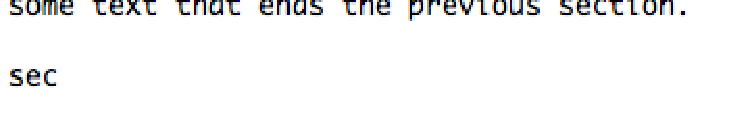
\includegraphics[width=3in]{figs/startsec}
\hfill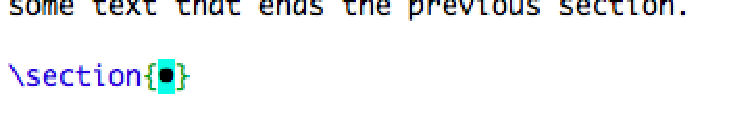
\includegraphics[width=3in]{figs/sec}}
\makebox[\textwidth]{
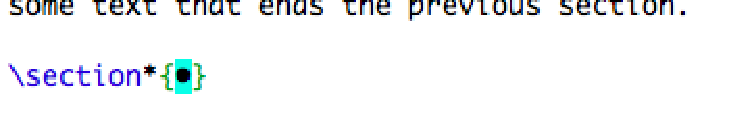
\includegraphics[width=3in]{figs/secs}
\hfill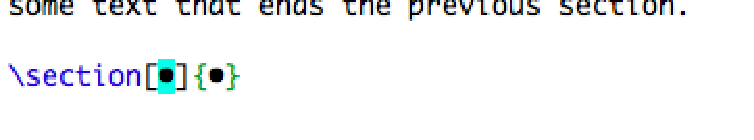
\includegraphics[width=3in]{figs/seco}}
\caption{Initially entered \texttt{sec} and successive pressings of \esckey\ from initial to last result before returning to the beginning. Corresponds to the sequence \texttt{initial}\(\to\)\texttt{sec}\(\to\)\texttt{secs}\(\to\)\texttt{seco}.}
\label{fig:sec}
\end{figure}

\subsection*{Environment Abbreviations}

Table (\ref{tbl:environments}) on page (\pageref{tbl:environments})  contains a list of abbreviations for different environments supplied in \CCT. Multiple vertically adjacent Environments with (almost) the same name correspond to variations in number and distribution of possible optional arguments or \texttt{*}-variants. There can also be more than one abbreviation for the same environment.

\subsection*{Commands \& Declarations}

As with Environments there are lots of variations with options and \texttt{*}-variants as well as multiple abbreviations corresponding to the same command. See Table (\ref{tbl:commands}) on page \pageref{tbl:commands}.

\subsection*{Greek Letters}

The Greek Letter abbreviations appear in Table (\ref{tbl:greek}) on page \pageref{tbl:greek}. There are `\texttt{xd}' (instead of just `\texttt{x}) versions of the greek letters that are used for in-line inclusion in text: \texttt{dxa} and \esckey\ produces \verb'\(\alpha\)' in the source and \(\alpha\) in a typeset line of text. These in-line equation, i.e., `\texttt{d}' versions of the letters are not shown in the table.

\begin{table}[!h]
\small
\centering
\caption{Environment abbreviations supplied in \CCT.}
\label{tbl:environments}
\vspace{10pt}
\begin{tabular}{llll}
\textbf{Abbreviation} & \textbf{Environment} & \textbf{Abbreviation} & \textbf{Environment} \\
\cmidrule[0.5pt](lr){1-1} \cmidrule[0.5pt](lr){2-2} \cmidrule[0.5pt](lr){3-3} \cmidrule[0.5pt](lr){4-4}\\
barr      & array       & blett   & letter \\
babs      & abstract    & blist   & list \\
bali      & align       & bminp   & minipage \\
balis     & align*      & bminpo  & minipage \\
baliat    & alignat     & bmult   & multline \\
baliats   & alignat*    & bmults  & multline* \\
balied    & aligned     & bpict   & picture \\
baliedat  & alignedat   & bpmat   & pmatrix \\
baliedato & alignedat   & bquot   & quotation \\
bapp      & appendix    & bquo    & quote \\
bbmat     & bmatrix     & bsplit  & split \\
bcase     & cases       & bsubeq  & subequations \\
bcent     & center      & btab    & tabular \\
bcenum    & compactenum & btabs   & tabular* \\
bcenumo   & compactenum & btabx   & tabularx \\
bcitem    & compactitem & btabl   & table \\
bcitemo   & compactitem & btablo  & table \\
bdes      & description & btabls  & table* \\
benu      & enumerate   & btablso & table* \\
benuo     & enumerate   & btbl    & table \\
bequ      & equation    & btblo   & table \\
bequs     & equation*   & btbls   & table* \\
beqn      & eqnarray    & btblso  & table* \\
beqns     & eqnarray*   & btabb   & tabbing \\
bfig      & figure      & bbib    & thebibliography \\
bfigo     & figure      & bindex  & theindex \\
bframe    & frame       & btheo   & theorem \\
bframeo   & frame       & btitpg  & titlepage \\
bflalig   & flalign     & btrivl  & trivlist \\
bflaligs  & flalign*    & bvarw   & varwidth \\
bfll      & flushleft   & bverb   & verbatim \\
bflr      & flushright  & bvers   & verse \\
bgath     & gather      & bwrap   & wrapfigure \\
bgaths    & gather*     & bwrapo  & wrapfigure \\
bgathed   & gathered    & bwrapo2 & wrapfigure \\
bgathedo  & gathered    & bwrapoo & wrapfigure \\
bite      & itemize     &         & \\
biteo     & itemize     &         & \\
\end{tabular}
\end{table}

\begin{table}[!h]
\small
\centering
\caption{Commands and Declarations in \CCT.}
\label{tbl:commands}
\vspace{10pt}
\makebox[\textwidth]{%
\begin{tabular}{llllll}
\textbf{Abbreviation} & \textbf{Command} & \textbf{Abbreviation} & \textbf{Command} & \textbf{Abbreviation} & \textbf{Command} \\
\cmidrule[0.5pt](lr){1-1} \cmidrule[0.5pt](lr){2-2} \cmidrule[0.5pt](lr){3-3} \cmidrule[0.5pt](lr){4-4} \cmidrule[0.5pt](lr){5-5} \cmidrule[0.5pt](lr){6-6}
\texttt{-{}-}    & textendash        & midr       & midrule        & renewcomo       & renewcommand \\
\texttt{-{}-{}-} & textemdash        & mnorm      & mathnormal     & renewcomoo      & renewcommand \\
\texttt{-{}-{}-} & textemdash w/sp   & msf        & mathsf         & rncm            & renewcommand \\
adlen            & addtolength       & mtt        & mathtt         & rnewc           & renewcommand \\
adcount          & addtocounter      & mit        & mathit         & rncmo           & renewcommand \\
bf               & textbf            & midr       & midrule        & rnewcoo         & renewcommand \\
bfd              & bfseries          & mnorm      & mathnormal     & rncmoo          & renewcommand \\
biblio           & bibliography      & mdd        & mdseries       & rmc             & rmfamily \\
bibstyle         & bibliographystyle & mbox       & mbox           & rbox            & raisebox \\
botr             & bottomrule        & makebox    & makebox        & rboxo           & raisebox \\
bibitem          & bibitem           & mboxo      & makebox        & rboxoo          & raisebox \\
bibitemo         & bibitem           & makebox    & makebox        & sec             & section \\
center           & centering         & mboxoo     & makebox        & secs            & section* \\
chap             & chapter           & mpar       & marginpar      & seco            & section \\
cmidr            & cmidrule          & multic     & multicolumn    & ssec            & subsection \\
cmidro           & cmidrule          & ncol       & space \& space & ssecs           & subsection* \\
em               & emph              & ncm        & newcommand     & sseco           & subsection \\ 
emd              & em                & newc       & newcommand     & sssec           & subsubsection \\
foot             & footnote          & ncmo       & newcommand     & sssecs          & subsubsection* \\
frac             & frac              & newco      & newcommand     & ssseco          & subsubsection \\
fbox             & fbox              & ncmoo      & newcommand     & spar            & subparagraph \\
fboxo            & framebox          & newcoo     & newcommand     & spars           & subparagraph* \\
fboxoo           & framebox          & nct        & newcolumntype  & sparo           & subparagraph \\
geometry         & geometry          & newct      & newcolumntype  & setl            & setlength \\
hw               & headwidth         & newpg      & newpage        & stcount         & stepcounter \\
hw2tw            & headw\(=\)textw   & npg        & newpage        & sf              & textsf \\
href             & href              & nline      & newline        & sfd             & sffamily \\
item             & item              & newlin     & newline        & sc              & textsc \\
ito              & item              & nlen       & newlength      & scd             & scshape \\
incg             & includegraphics   & newlen     & newlength      & sl              & textsl \\
incgo            & includegraphics   & nenv       & newenvironment & sld             & slshape \\
it               & textit            & newenv     & newenvironment & sqrt            & sqrt \\
itd              & itshape           & nenvo      & newenvironment & sqrto           & sqrt \\
latex            & LaTeX             & newenvo    & newenvironment & tt              & texttt \\
latexs           & LaTeX w/sp        & nenvoo     & newenvironment & ttd             & ttfamily \\
latexe           & LaTeXe            & newenvoo   & newenvironment & tw              & textwidth \\
latexes          & LaTeXe w/sp       & pgref      & pageref        & tex             & TeX \\
label            & label             & par        & paragraph      & texs            & TeX w/sp \\
lbl              & label             & pars       & paragraph*     & tilde           & textasciitilde \\
lettrine         & lettrine          & paro       & paragraph      & topr            & toprule \\
lettrineo        & lettrine          & pgs        & pagestyle      & toc             & tableofcontents \\
listf            & listoffigures     & parbox     & parbox         & tableofcontents & tableofcontents \\
listt            & listoftables      & parboxo    & parbox         & tpgs            & thispagestyle \\
rule             & rule              & parboxoo   & parbox         & thispagestyle   & thispagestyle \\
ruleo            & rule              & parboxooo  & parbox         & up              & textup \\
mbf              & mathbf            & pbox       & parbox         & upd             & upshape \\
mrm              & mathrm            & pboxo      & parbox         & url             & url \\
mcal             & mathcal           & pboxoo     & parbox         & usep            & usepackage \\
msf              & mathsf            & pboxooo    & parbox         & usepo           & usepackage \\
mtt              & mathtt            & ref        & ref            & verb            & verb \\ 
mit              & mathit            & renewcom   & renewcommand   & verb2           & verb \\
\end{tabular}
}
\end{table}

\begin{table}[!h]
\small
\centering
\caption{Greek Letters in \CCT. The `\texttt{d}' versions are not shown.}
\label{tbl:greek}
\vspace{10pt}
\begin{tabular}{llll}
\textbf{Abbreviation} & \textbf{Command} & \textbf{Abbreviation} & \textbf{Command} \\
\cmidrule[0.5pt](lr){1-1} \cmidrule[0.5pt](lr){2-2} \cmidrule[0.5pt](lr){3-3} \cmidrule[0.5pt](lr){4-4}
xa  & alpha      & xph  & phi \\
xb  & beta       & xcph & Phi \\
xch & chi        & xvph & varphi \\
xd  & delta      & xps  & psi \\
xcd & Delta      & xcps & Psi \\
xe  & epsilon    & xs   & sigma \\
xve & varepsilon & xcs  & Sigma \\
xet & eta        & xvs  & varsigma \\
xg  & gamma      & xz   & zeta \\
xcg & Gamma      & xr   & rho \\
xio & iota       & xvr  & varrho \\
xl  & lambda     & xt   & tau \\
xcl & Lambda     & xth  & theta \\
xm  & mu         & xcth & Theta \\
xn  & nu         & xvth & vartheta \\
xo  & omega      & xu   & upsilon \\
xco & Omega      & xcu  & Upsilon \\
xp  & pi         & xx   & xi \\
xcp & Pi         & xcx  & Xi \\
xvp & varpi      &      & \\
\end{tabular}
\end{table}


\end{document}
